%
% -- Manlio Modugno

\documentclass{beamer} 
\usepackage{eulervm}
%\usepackage{booktabs}
\usepackage{listings}
\usepackage{bold-extra}
\usepackage{cancel}
\usepackage{fancybox}
\usepackage{soul}
\usepackage[english]{babel}
\usepackage[utf8]{inputenc}
\usepackage{hyperref}
\usepackage{amsmath}
%\hypersetup{colorlinks=true,urlcolor=blue}

\newcommand{\codefont}{\fontsize{6}{8}\selectfont}
\lstset{language=[Sharp]C, 
captionpos=b, 
frame=lines,
lineskip= 1pt, %space between lines
basicstyle=\codefont, 
keywordstyle=\color{blue}, 
commentstyle=\color{green}, 
stringstyle=\color{red}, 
numbers=left, 
numberstyle=\tiny, 
stepnumber=2,
numbersep=5pt,
breaklines=true, 
breakatwhitespace=false,
showstringspaces=false,
frame=single,
tabsize=2,
emph={double,bool,int,unsigned,char,true,false,void},
emphstyle=\color{blue},
emph={Assert,Test},
emphstyle=\color{red},
emph={[2]\using,\#define,\#ifdef,\#endif},
emphstyle={[2]\color{blue}}
}


\mode<presentation>
\definecolor{title_color}{RGB}{2,128,181} 
\usetheme{Ilmenau}
\usecolortheme[named=title_color]{structure}
\setbeamercolor{palette quaternary}{use=structure,fg=black,bg=white} %header footer color
\useoutertheme[subsection=false]{smoothbars}
\setbeamercovered{transparent}
\setbeamertemplate{navigation symbols}{}
\setbeamerfont{subsection in toc}{size=\scriptsize}

\title{Sequence Diagram + Refactoring chapter 1}
\author{Manlio Modugno}
\institute[GMTechnologies] 

\date[30.06.2016] 
{30.06.2016 - Sequence Diagram + Refactoring chapter 1}

\subject{}

\graphicspath{{img/}}
\pgfdeclareimage[height=0.6cm]{mfg-logo}{img/mfgLogo}
\logo{\pgfuseimage{mfg-logo}}

%
% Content start
%
\begin{document}
\begin{frame}
  \titlepage
\end{frame}

\begin{frame}
  \frametitle{Argomenti Trattati}
  \tableofcontents
\end{frame}

\section{Sequence Diagram}
\subsection{Basics}
\begin{frame}
  \frametitle{Basics}
  \begin{itemize}
  		\item<+-> Define event sequences that result in some desired outcome
		\item<+-> Focus is on the order in which messages occur
		\item<+-> Vertical dimension: shows (top down) the time sequence of messages
		\item<+-> Horizontal dimension: shows (left right) the objects involved in the messages communication
  \end{itemize}
\end{frame}

\subsection{Lifeline}
\begin{frame}
	\frametitle{Lifeline}
	\begin{center}
		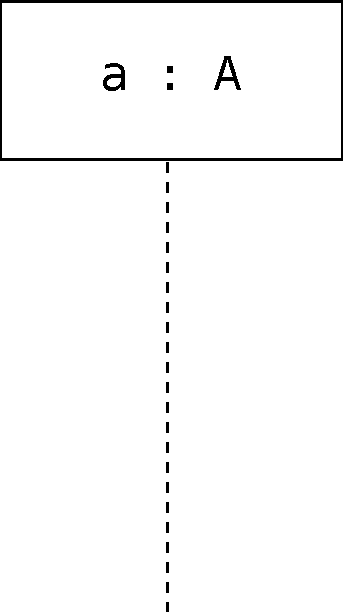
\includegraphics[scale=0.4]{box}
	\end{center}
	\textbf{Note:}
	\begin{itemize}
  			\item Drown as a box with a dashed line.
  			\item Name is inside the box in the form $\Rightarrow$ instance/role name [optional] : Class Name
  			\item Instances are underlined, role not.
	\end{itemize}
\end{frame}

\subsection{Messages}
\begin{frame}
	\frametitle{Messages}
	\begin{center}
		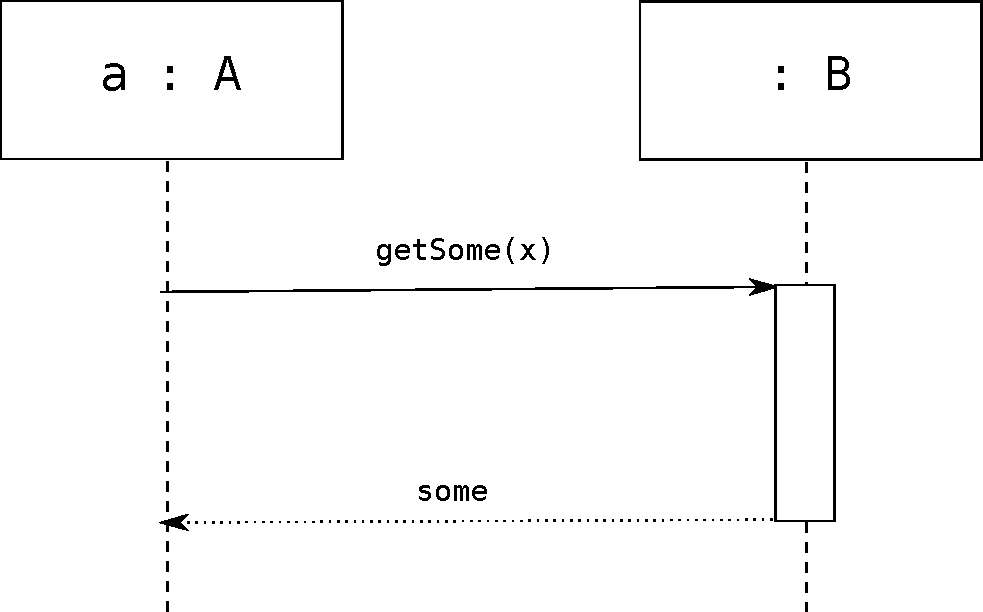
\includegraphics[scale=0.35]{messages}
	\end{center}
	\textbf{Note:}
	\begin{itemize}
  			\item Messages depicted as arrowhead lines 
  			\item Message name placed above the arrowed line
  			\item Message sent on a receiving object is a method that the receiving object's class implements.
  			\item Dotted arrowhead represent return value [optional]
	\end{itemize}
\end{frame}

\subsection{Guards}
\begin{frame}
	\frametitle{Guards}
	\begin{center}
		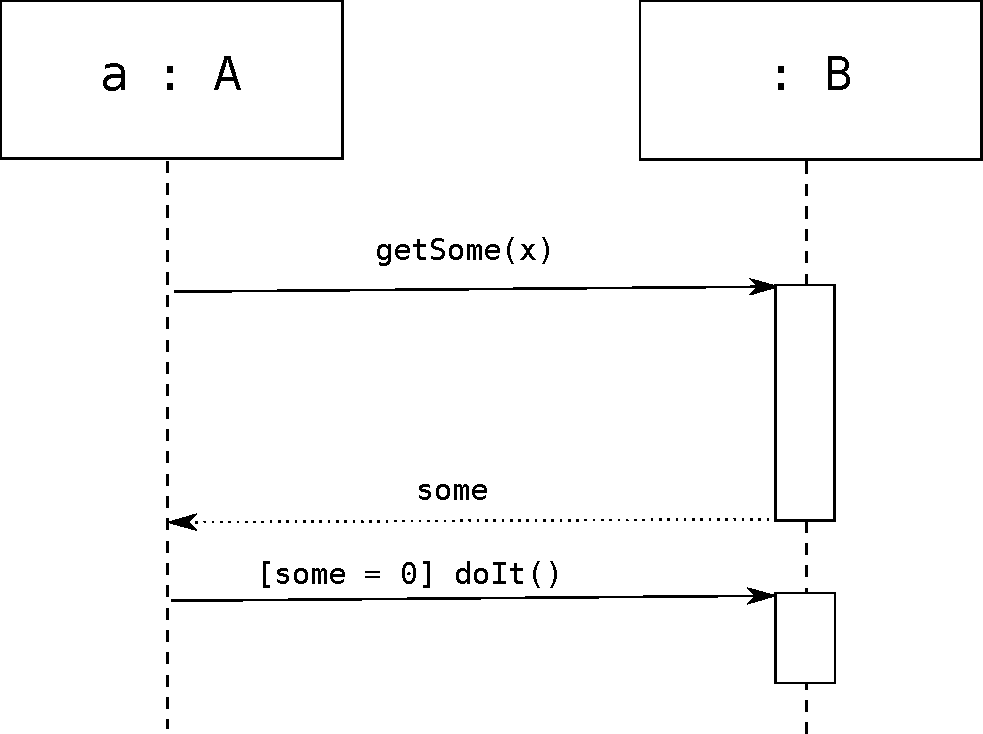
\includegraphics[scale=0.35]{guards}
	\end{center}
	\textbf{Note:}
	\begin{itemize}
  			\item When a condition must be met for a message to be sent
  			\item If some = 0 doIt() message is sent to B
	\end{itemize}
\end{frame}

\subsection{Combined fragments}
\begin{frame}
	\frametitle{Combined fragments: alternatives / options / loops}
	\begin{center}
		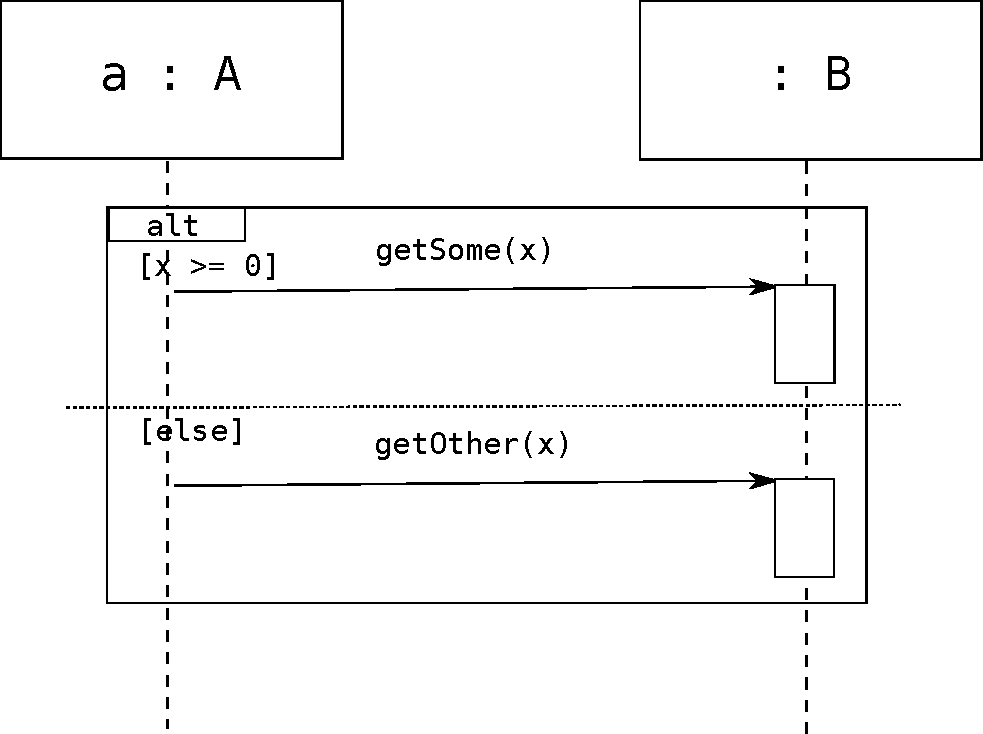
\includegraphics[scale=0.25]{alt}
	\end{center}
	\textbf{Note:}
	\begin{itemize}
  			\item Used to group sets of messaged together to show conditional flow
  			\item \textbf{Alternatives:} models if then else conditional with label ``alt'' and optional guards
  			\item \textbf{Options:} models if then conditional with label ``opt''
  			\item \textbf{Loops:} models a repetitive sequence with label ``loop'' and optional guard
	\end{itemize}
\end{frame}

\section{Refactoring, First Example}
\subsection{Description}
\begin{frame}
  \frametitle{Refactoring, First Example: description}
  \begin{itemize}
  		\item Rafactor an existing program that calculate and print a statement of a customer's charges in a video store
		\item Program keeps track of customer's movies and for how long he rented
		\item Charges depend on rent time and on movie's types (using renter points)
  \end{itemize}
\end{frame}

\subsection{Classes}
\begin{frame}
  \frametitle{Classes}
  \begin{itemize}
  		\item Movie
		\item Rental
		\item Customer
  \end{itemize}
\end{frame}

\subsection{Concepts}
\begin{frame}
  \frametitle{Concepts / Comments}
  \begin{itemize}
  		\item<+-> Is a simple program that don't change? It can works..does not really matter..
		\item<+-> ..but if is a fragment of a more complex system.. we have problems!
		\item<+-> ..and they arise when we want \textbf{to change} the program!
		\item<+-> Compiler doesn't care about the code (actualy it can..).. humans care! (Remember Reeves?)
		\item<+-> \textbf{Poorly designed systems are hard (i.e. expensive) to change}
  \end{itemize}
\end{frame}

\begin{frame}
  \frametitle{Rules}
  \begin{itemize}
  	\item If program's code is not structored in a convenient way to add a new feature.. \textbf{first refactor then add the feature!}
  	\item  Build a solid set of tests for the section code you're going to refactor.. they assure that you aren't changing original behaviour.. 
  	\item Proceed with small steps!
    \end{itemize}
\end{frame}

\subsection{Change requirements}
\begin{frame}
  \frametitle{New Requirements}
  \begin{itemize}
  		\item Statement in html
		\item New / Different charging rules
		\item Change the way how users classify movies.. they don't know how yet!
  \end{itemize}
\end{frame}

\subsection{Moves}
\begin{frame}
  \frametitle{First Step in Refactoring: attack statement method}
   \begin{itemize}
  		\item Contains almost the whole logic of the program
		\item It's really long
		\item Decomposing in smaller parts $\Rightarrow$ tend to make things more manageable..
		\item Aim is to produce html statement with much less duplication
  \end{itemize}
\end{frame}

\begin{frame}[containsverbatim]
	\frametitle{Extract Method}
	Start from switch staement \\
	\begin{lstlisting}
...
//determine amounts for each line
switch (each.getMovie().getPriceCode()) {
	case Movie.REGULAR:
		thisAmount += 2;
		if (each.getDaysRented() > 2)
		thisAmount += (each.getDaysRented() - 2) * 1.5;
	break;
	case Movie.NEW_RELEASE:
		thisAmount += each.getDaysRented() * 3;
	break;
	case Movie.CHILDRENS:
		thisAmount += 1.5;
		if (each.getDaysRented() > 3)
		thisAmount += (each.getDaysRented() - 3) * 1.5;
	break;
}
...
\end{lstlisting}
\end{frame}

\begin{frame}
  \frametitle{Extract Method}
  \textbf{To avoid bug introduction we must proceed in a safe way:}
   \begin{itemize}
  		\item Identify any variables (local and parameters) local in scope of the code block. (each and thisAmount in the example)
		\item Any not-modified variables can be passed as parameter to the extracted method
		\item Modified variables need more care. In this case tisAmount is retuened from the extracted method
		\item ...		
		\item Some IDEs offer automatic tool to apply some refactor moves
  \end{itemize}
\end{frame}

\begin{frame}[containsverbatim]
	\frametitle{Extract Method}
	Extracted method \\
	\begin{lstlisting}
public String statement() { ...thisAmount = amountFor(each);...}
private double amountFor(Rental each) {
	double thisAmount = 0;
	switch (each.getMovie().getPriceCode()) {
		case Movie.REGULAR:
			thisAmount += 2;
			if (each.getDaysRented() > 2)
				thisAmount += (each.getDaysRented() - 2) * 1.5;
		break;
		case Movie.NEW_RELEASE:
			thisAmount += each.getDaysRented() * 3;
		break;
		case Movie.CHILDRENS:
			thisAmount += 1.5;
			if (each.getDaysRented() > 3)
				thisAmount += (each.getDaysRented() - 3) * 1.5;
		break;
	}
	return thisAmount;
}
\end{lstlisting}
\end{frame}

\begin{frame}[containsverbatim]
  \frametitle{Renaming}
   \begin{itemize}
     \item Good code should communicate what is doing clearly $\Rightarrow$ variable names are a key to clear code
   \item  ``Any fool can write code that a computer can understand. Good programmers write
code that humans can understand.''
	\end{itemize}
	\begin{lstlisting}
	private double amountFor(Rental aRental) {
		double result = 0;
		switch (aRental.getMovie().getPriceCode()) {
		...
	\end{lstlisting}
\end{frame}

\begin{frame}[containsverbatim]
  \frametitle{Move Method}
  \textbf{In most cases a method should be on the object whose data it uses}
   \begin{itemize}
  		\item The extracted method lies in Customer class, but it use no information of the class..
		\item ..so move it in class Rental
  \end{itemize}
  \begin{lstlisting}
	class Rental {
		double getCharge() {
			double result = 0;
			switch (getMovie().getPriceCode()) {
				...
			}
		}
	}
	\end{lstlisting}
\end{frame}

\begin{frame}[containsverbatim]
  \frametitle{Replace temp with query}
  \textbf{Temp variables can ba a problem:}
   \begin{itemize}
  		\item They can cause a lot of parameters to be passed around and you can easily lose track on the reason they are in a given place..
		\item In a long method they can be insidious.. reassignement, tackle parameters move, ..
		\item Pay attention on performance (double call in this case), but \textbf{don't optimize prematurely!} (more on that in next charpter)
  \end{itemize}
  \begin{lstlisting}
  	//thisAmount = each.getCharge()
	...
	//show figures for this rental
	result += "\t" + each.getMovie().getTitle()+ "\t" +
	String.valueOf(each.getCharge()) + "\n";
	totalAmount += each.getCharge();
	...
	\end{lstlisting}
\end{frame}

\begin{frame}
  \frametitle{Continue}
  \textbf{Apply similar moves on ``Frequent Renter Points''.. }
     \begin{itemize}
  		\item Note \textit{Removing Temps} on getTotalCharge() and getTotalFP() $\Rightarrow$ increase code, but isolate logic from presentation
  		\item Note also that code increase because of tech limit of Java (functional can do better here..)
  		\item Don't bother (again) about performance.. we have to profile!
  	\end{itemize}
  	\begin{center}
		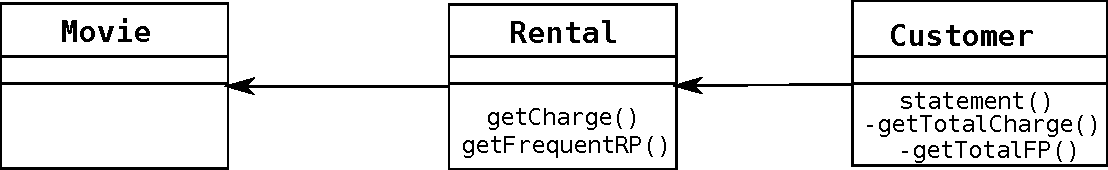
\includegraphics[scale=0.5]{refactorApply}
	\end{center}
\end{frame}

\end{document}